\chapter{Descripción} \label{cap:Descripcion}
%\section{Descripción de la herramienta SLAM-Test-Bed} \label{s:descripcionHerramienta}
En este capítulo describiremos en detalle el funcionamiento de la herramienta SLAM-Test-Bed

La herramienta SLAM-Test-Bed consta de un entorno gráfico para realizar comparaciones sobre datasets obtenidos tras aplicar algoritmos SLAM. 
Nos permitirá medir la exactitud de los resultados de la aplicación de un algoritmo con los resultados de otro algoritmo o comparar varios resultados de un mismo algoritmo en el que se han aplicado distintos parámetros de ejecución.
La herramienta cuenta de un interfaz gráfico en 3D desarrollado con QT y la librería Eigen.


Mediante un interfaz gráfico permite realizar transformaciones a un conjunto de datos de entrada, representar gráficamente en 3d la nube de puntos ground truth, el conjunto de datos transformado y el conjunto de datos estimados.
También permite hacer giros zoom sobre las nubes de puntos
Entre las transformaciones permiten hacer cambios en 
ESCALA
TRASLACIONES en ejes X,Y,Z
ROTACIONES en ejes X,Y,Z
Offset de tiempo
Interpolación
Ruido gaussiano
Ruido Cósmico
[imgTransformaciones]
\begin{figure}[H]
\begin{center}
\subfigure[]{\label{fig:transformaciones}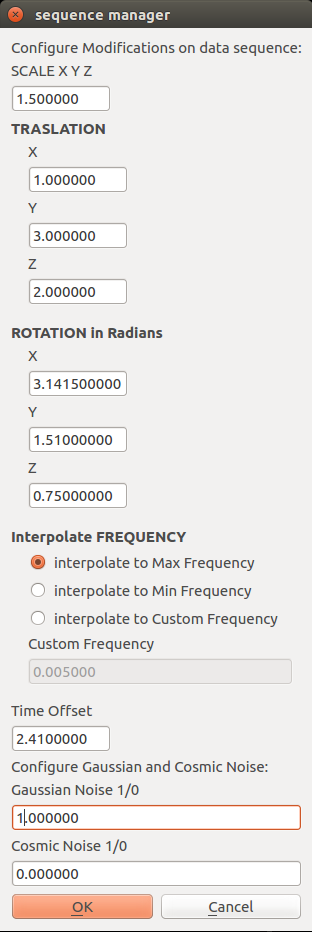
\includegraphics[height=12.0cm,width=4.0cm]{img/cap5/imgTransformaciones.png}}
\hspace{0.5cm}
%\subfigure[]{\label{fig:LG_hombot}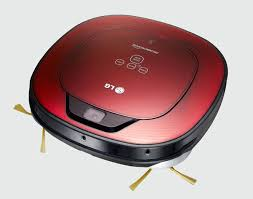
\includegraphics[height=6.0cm]{img/cap2/LG_hombot.jpg}}
\end{center}
%\caption{Robot Dyson 360 Eye (a) Robot Roomba 966 (b) Robot Hombot de LG (c).}
\caption{Sentido de la estimación , A to B o B to A }
\end{figure}

El formato del conjunto de datos ground-truth será timestamp, posición x, posición y, posición z

Posteriormente tras aplicar las transformaciones definidas en el interfaz gráfico sobre el ground truth, la herramienta devolverá los resultados de estimar dichas transformaciones.


A continuación describiremos en detalle las transformaciones permitidas por la herramienta

\textbf{Escala}. Permite modificar los datos de entrada a nivel de escala. La escala siempre será mayor que cero y se admitirán números con reales

\textbf{Traslaciones}. Se podrán definir traslaciones sobre cada uno de los 3 ejes de coordenadas. 
La traslación admite números reales positivos y negativos.

\textbf{Rotaciones}. Se podrán definir rotaciones sobre cada unos de los 3 ejes de coordenadas. El valor de cada rotación se insertará en Radianes. Los valores admitidos serán números reales tanto positivos como negativos

\textbf{Offset de tiempo}. Con el offset de tiempo podremos introducir un gap en los valores de timestamp del fichero de entrada que más tarde podremos estimar. La exactitud del offset será de centésimas, es decir con 2 decimales

\textbf{Interpolación}: Se podrán realizar 3 tipos de interpolación de los datos.
	Interpolación a la frecuencia máxima
	Interpolación a la frecuencia mínima
	Interpolación a frecuencia personalizada

\textbf{Ruido Gaussiano}: Una de las transformaciones que podremos aplicar sobre el conjunto de datos del groundtrouth es aplicar un ruido gaussiano a los datos transformados

\textbf{Ruido Cósmico}: Otra transformación a aplicar sobre los datos transformados es la incorporación del ruido cósmico

\textbf{Menu de estimaciones}:
Una vez hemos aplicado las transformaciones sobre el groundtrouh, se generará como resultado un nuevo dataset, el transformado.
El menú gráfico nos permitirá estimar que transformaciones se han realizado, y se podrán estimar en 2 sentidos de aplicación.

\begin{figure}
\begin{center}
\subfigure[]{\label{fig:menu A to B y B to A}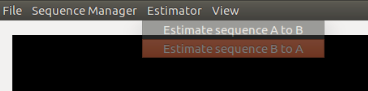
\includegraphics[height=3.0cm,width=8.0cm]{img/cap5/menuAtoB_BtoA.png}}
\hspace{0.5cm}
%\subfigure[]{\label{fig:LG_hombot}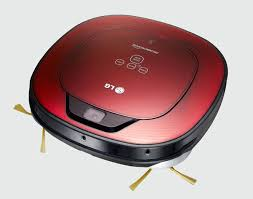
\includegraphics[height=6.0cm]{img/cap2/LG_hombot.jpg}}
\end{center}
%\caption{Robot Dyson 360 Eye (a) Robot Roomba 966 (b) Robot Hombot de LG (c).}
\caption{Transformaciones permitidas sobre el dataset de entrada }
\end{figure}
	Desde el groundtrouth estimar que transformaciones se han aplicado para llegar a la secuencia de datos transformadados. ( A To B)

	Desde la secuencia transformada estimar las transformaciónes para obtener el groundtrouth . ( B to A)
Estas 2 estimaciones se han realizado aplicando cálculos matemáticos tipo SVD y PCA sobre las matrices de datos

\textbf{Otras particularidades del menú gráfico}:
	Unir todos los puntos del dataset 
    
    Visualizarlos como datos individuales

	visualizar sólo los datos estimados.


